\begin{titlepage}

\begin{center}
  \Huge
  ELT4 - Vorlesungsnotizen

\vspace{1cm}
\normalsize
\usepgflibrary{arrows}

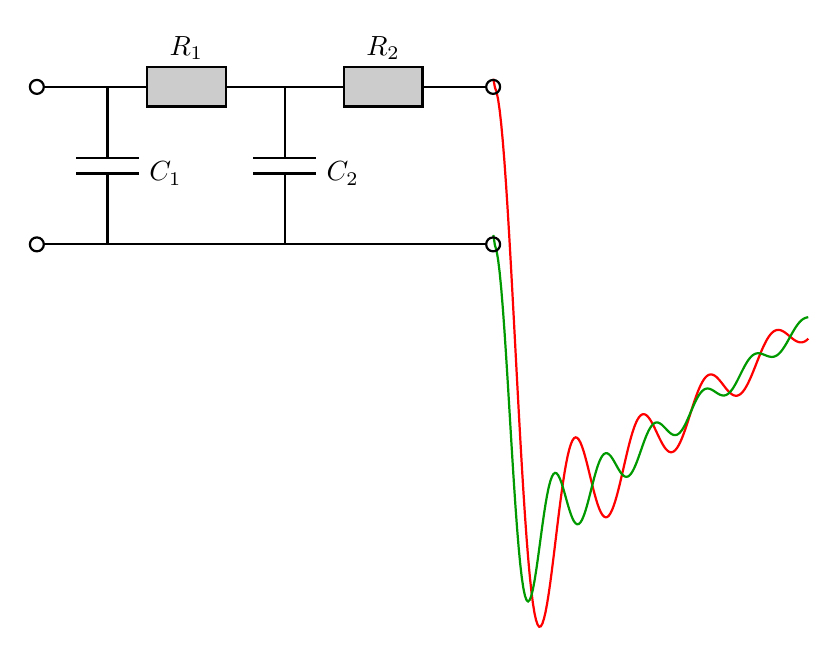
\begin{tikzpicture}[]

\coordinate (O) at (0,0,0);


% Koordinatensystem
%\begin{scope}[thick, ->,
%  x={(1cm,0cm)}, 
%  y={(-0.38cm,-0.38cm)}, 
%  z={(0cm,1cm)}
%]
%  \draw (O) -- +(2,0,0) node[right] {$x$};
%  \draw (O) -- +(0,2,0) node[below] {$y$};
%  \draw (O) -- +(0,0,2) node[above] {$z$};
%  \draw (O) -- +(-2,0,0) node[left] {$-x$};
%  \draw (O) -- +(0,-2,0) node[above] {$-y$};
%  \draw (O) -- +(0,0,-2) node[below] {$-z$};
%\end{scope}


% Plot der beiden Funktionen
\begin{scope}[thick,
  x={(1cm, 0cm)},
  x={(0.4cm,0.3cm)},
  z={(0cm,1cm)},
  xshift = -3.1cm,
  yshift = -6cm
]
 \draw[color=red, samples=200, domain=0.0001:10]
    plot (\x, {2*sin((3*\x) r) / \x});
  \draw[color=green!60!black, samples=200, domain=0.0001:10]
    plot(\x, {sin((4*\x) r) / \x});
\end{scope}

% Schaltung
\begin{scope}[
 thick, 
 rotate around={0:(-5,0)}, 
 xscale=1,
 fill opacity=0.2,
 text opacity= 1
]
  \draw[o-] (-9,0) -- +(1.5,0);
  \draw[fill] (-7.5,-0.25) rectangle node[above=6] {$R_1$} (-6.5,0.25);
  \draw (-6.5,0) -- (-5,0);
  \draw[fill] (-5,-0.25) rectangle node[above=6] {$R_2$} (-4,0.25);
  \draw[-o] (-4,0) -- (-3,0);.

  % Kondensator C1
  \draw (-8,0) -- +(0,-0.9);
  \draw (-8.4, -0.9) -- +(0.8,0);
  \draw (-8.4, -1.1) -- +(0.8,0) node [right] {$C_1$};  
  \draw (-8,-1.1) -- + (0,-0.9);


  \draw (-5.75,0) -- +(0,-0.9);
  \draw (-6.15, -0.9) -- +(0.8,0);
  \draw (-6.15, -1.1) -- +(0.8,0) node [right] {$C_2$};  
  \draw (-5.75,-1.1) -- + (0,-0.9);

  % Unterer Pfad
  \draw[o-o] (-9,-2) -- +(6,0);

\end{scope}
\end{tikzpicture}

\vfill

Jürg Rast \& Gian Claudio Köppel, \today

\end{center}

\end{titlepage}